%___________________________________________
%*************************************************************
% Level Playing
%___________________________________________
%^^^^^^^^^^^^^^^^^^^^^^^^^^^^^^^^^^^^^^^^^^^^^^^^^^^

\section{Level Playing Module}

The main purpose of the level playing module is to evaluate the fitness of agents during the learning process. An effective learning process needs a diverse testbed, thus the level playing module must be deterministic, highly configurable and able to provide variety. 

%-----------------------------------------------------------------------
% Design
%-----------------------------------------------------------------------

\subsection{Design}

\begin{figure}[t]
	\centering
	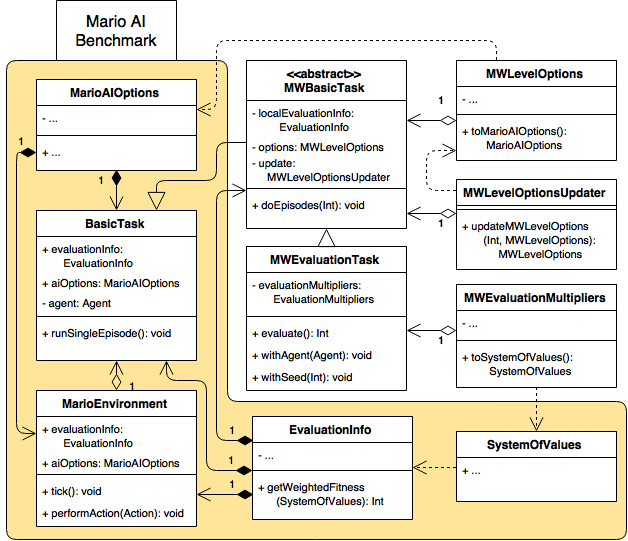
\includegraphics[scale=0.5]{PlayingClassDiagram.png}
	\caption{UML class diagram of the level playing module.}
	\label{fig:pumlcd}
\end{figure}

In the benchmark the heart of the game engine is the \emph{MarioEnvironment} class. It is responsible for calling the \emph{LevelGeneration} class, updating the scene each tick with an action, and reporting the scene through the Environment interface. Parameters controlling level generation and playing are contained in the \emph{MarioAIOptions} class. The \emph{BasicTask} class controls the game loop in conjunction with an agent. It initialises the MarioEnvironment class with options, then runs through the loop, commanding a tick, passing the environment to the agent and finally requesting an action and passing it to the MarioEnvironment instance. Statistics pertaining to the agents performance are stored in MarioEnvironment in the \emph{EvaluationInfo} class, which are cloned to BasicTask at the end of the level. Fitness can be requested from EvaluationInfo with the optional parameter, a \emph{SystemOfValues} instance, which contains the multipliers for various measurements.

The MarioAIOptions class contains several useful parameters. They include: a integer seed, which is passed to the level generator's RNGs; a boolean that toggles visualisation; integers that determine level difficulty, length and time-limit; and booleans that toggle enemies, pits and blocks. The SystemOfValues class contains multipliers for  distance achieved, whether or not the level was completed, the amount of time left on completion as well as many others.

\vspace{\baselineskip}

The level playing module will extend this system. Its primary objective will be to allow for multiple levels (episodes) to be played with options that update as prescribed by some parameter class. Upon completion it will produce a fitness based on all levels played. Furthermore, it will allow for the injection of different agents and level seeds, to allow different agents to play the same options without rebuilding the instance. A UML class diagram for the module can be found in Figure \ref{fig:pumlcd}.

Level options are stored in the \emph{MWLevelOptions} class, which acts as an adapter for the MarioAIOptions class. Each new level these will be updated by the dedicated \emph{MWLevelOptionsUpdater} class. The \emph{EvaluationMultipliers} class is an adapter for the SystemOfValues class, which is used to calculate the fitness at the end of a sequence of levels. These classes are separated from the the game playing task and are included using constructor dependency injection. This helps to decouple the system and improve the ability to modify and test.

Both MWLevelOptions and EvaluationMultipliers are designed to be data classes, which provides determinism and thread safety, as well as easy persistence. MWLevelOptionsUpdater's qualities in this regard are Implementation details and are discussed in a following section. The full list of parameters held in these classes can be found in the Appendix !REF!.


%-----------------------------------------------------------------------
% Implementation
%-----------------------------------------------------------------------

\subsection{Implementation}

\subsubsection{Parameter Classes}
\label{subsec:paramclasses}

The MWLevelOptions and MWEvaluationMultipliers classes were implemented as data classes in an immutable builder pattern style. Each field has a \emph{withField(field)} method that returns a cloned instance with that field changed. This affords a concise, declarative style, whilst maintaining immutability. MWEvaluationMultipliers has a implicit converter to a SystemOfValues instance, which is required for evaluation in the benchmark. However, a similar approach was not possible for converting MWLevelOptions to a MarioAIOptions instance (required for the game-engine). MarioAIOptions hold more parameters than MWLevelOptions (e.g. agent and level seed), therefore the adapter function takes both the current MarioAIOptions and a MWLevelOptions instance as parameters and updates the former by overriding the corresponding fields with values from the latter. A full list of field for both the MWLevelOptions and MWEvaluationMultipliers classes can be found in Appendix \ref{app:loem}.

MWLevelOptions was not implemented as a class. Instead, MWBasicTask expects a lambda function. This lambda takes the episode number and the current MWLevelOptions, returning an updated set of options. MWLevelOptions builder structure ensures this is always a new instance, and hence maintains immutability. The inclusion of the episode number allows the function to remain deterministic. Moreover, with the ability to build closures in Scala, this lambda can be built from data (for example, a list of options, where indexes relate to episode number).

\subsubsection{Persistence}
\label{subsec:evalparams}

The primary use of the level playing module is during the evaluation stage of the learning process. Hence, it was decided to use ECJ's parameter file system to persist level playing parameters, which allows them to be written in the same file as the rest of the learning parameters.

ECJ's parameter system builds upon Java's Properties file system. From a parameter file (formatted in the Java Properties format) a ParameterDatabase can be built, from which specific parameters can be requested using the Parameter class. This system was used to persist the two parameter classes, MWLevelOptions and MWEvaluationMultipliers; the level options update lambda data; and other level playing data such as number of levels (episodes) and base level seed. For example, the following lines would set the number of levels to 10 and the base difficulty to 5:

\begin{minipage}{0.9\linewidth}
\centering
\begin{lstlisting}
          level.num-levels = 10
level.base.difficulty-num = 5
\end{lstlisting}
\end{minipage}

A static utility class EvaluationParamsUtil was created to handle the reading of the level playing data from these files. A ParameterDatabase is built and passed to utility class, which builds the required parameter class. For MWLevelOptions and MWEvaluationMultipliers it searches for the prefixes `{\ttfamily level.base}' and `{\ttfamily mult}' respectively and then looks for suffixes corresponding to specific fields. If a field's suffix is not found then it is initialised to a default value (which is always zero for MWEvaluationMutlipliers).

The update lambda is built as a closure on a collection of Map instances, one for each field in MWLevelOptions. For each {\ttfamily n} from 0 to the number of levels (episodes), the utility function looks for the prefix `{\ttfamily level.\{n\}}', which is used to hold the update for episode \textbf{n}. For each field a Map is built and using the same suffixes as for MWLevelOptions, key-value pairs are added mapping \textbf{n} to the value found. When the update lambda is called, it consults these maps and updates the MWLevelOptions with the new value if one is found for the current episode number.

For example, if the parameter file contained the following lines:

\begin{minipage}{0.9\linewidth}
\centering
\begin{lstlisting}
   level.num-levels = 4
 level.base.enemies = false
    level.1.enemies = true
    level.3.enemies = false
\end{lstlisting}
\end{minipage}

Then enemies would be off for the first episode, on for the second and third and off again for the fourth and final episode.

\subsubsection{The Episode Loop}

The entry point of the level playing module is the MWEvaluationTask class, which extends the abstract MWBasicTask class. MWEvaluationTask is instantiates with a base set of options (as MWLevelOptions), a MWEvaluationMutlipliers instance and an update lambda, as well as the number of episodes (levels) to run. The agent and base level seed can be injected with the \emph{withAgent(agent)} and \emph{withLevelSeed(seed)} methods (which also reset of evaluation information).

\begin{minipage}{0.9\linewidth}
\centering
\begin{lstlisting}[language=scala]
class MWEvaluationTask(val numberOfLevels: Int, 
                       val evalValues: MWEvaluationMultipliers, 
                       override val baseLevelOptions: MWLevelOptions, 
                       override val updateOptionsFunc: (Int, MWLevelOptions) => MWLevelOptions)
                           extends MWBasicTask("MWMainPlayTask", baseLevelOptions, updateOptionsFunc, visualisation, args) with EvaluationTask {

    private var baseLevelSeed: Int = 0;
    
    override def nextLevelSeed(episode: Int, lastSeed: Int) =  {
        (3*episode) + lastSeed
    }    
        
    override def evaluate: Int = {
        doEpisodes
        localEvaluationInfo.computeWeightedFitness(evalValues)
    }
  
    override def withAgent(agent: Agent): MWEvaluationTask = {
        super.injectAgent(agent, true)
        this
    }
\end{lstlisting}
\end{minipage}     
    
\begin{minipage}{0.9\linewidth}
\centering
\begin{lstlisting}[language=scala]   
    override def withLevelSeed(seed: Int): MWEvaluationTask = {
        baseLevelSeed = seed
        super.injectLevelSeed(seed, true)
        this
    }
}
\end{lstlisting}
\end{minipage}  

On calling the \emph{evaluate()} method, the number of levels is passed to the \emph{doEpisodes(numberOfEpisode)} (a superclass method), which loops as follows:

\begin{minipage}{0.9\linewidth}
\centering
\begin{lstlisting}[language=scala]

def doEpisodes(amount: Int): Unit = {
    @tailrec
    def runSingle(iteration: Int, prevOptions: MWLevelOptions, disqualifications: Int): Int = {
        if (iteration == amount) { 
            disqualifications
        } else {
            // Calls the update lambda to get episodes set of options
            val newOptions = updateOptions(iteration, prevOptions)
            
            // Converts options to class required for game-engine
            val marioAIOptions = MWLevelOptions.updateMarioAIOptions(super.options, newOptions)
            
            // Updates the level seed (which is set to increase each episode by MWEvaluationClass)
            // Agent instance is already being held here
            marioAIOptions.setLevelRandSeed(nextLevelSeed(iteration, marioAIOptions.getLevelRandSeed))
            
            // Resets the evaluation information in the super class
            super.setOptionsAndReset(marioAIOptions)
\end{lstlisting}
\end{minipage}

\begin{minipage}{0.9\linewidth}
\centering
\begin{lstlisting}[language=scala]
            // Generates and runs the level using the super class
            // Returns true if the agent was not disqualified (took too long to return an action)
            val notDisqualified: Boolean = runSingleEpisode(1)
            val disqualification: Int = if (!notDisqualified) 1 else 0
       
            // Update the evaluation information for the entire run
            // (as the super classes evaluationInfo gets reset every level
            updateLocalEvaluationInfo(super.getEvaluationInfo)
            
            // Loop
            runSingle(iteration+1, newOptions, disqualifications + disqualified)
        }
    }
    
    // Sets the base options
    super.setOptionsAndReset(MWLevelOptions.updateMarioAIOptions(options, baseLevelOptions))
    disqualifications = runSingle(0, baseLevelOptions, 0)
}
\end{lstlisting}
\end{minipage}


Before every episode the options are updated by the lambda, updating the base options in the first episode. A new level seed is also requested from the MWEvaluationClass, which simply increases it each episode. These updates are converted and added to a MarioAIOptions instance and passed to the superclass in the benchmark. A single level is then generated and played using the superclass. Evaluation information is added to MWBasicTask's local evaluation information (as the former is reset every episode) and the function loops tail recursively.

When the number of loops equals the number of levels the function exits. At this point the \emph{evaluate()} method requests a fitness from the local evaluation information, passing in the evaluation multipliers, which is then returned.

%-----------------------------------------------------------------------
% Benchmark Edit
%-----------------------------------------------------------------------

\subsection{Modifying the Benchmark}
\label{subsec:enginemod}

Preliminary runs of the benchmark software revealed several issues and defects. As the learning algorithm would run over several generations, any errors could halt it prematurely, which could be costly in terms of project time keeping. In order to address this a Java project was created from the benchmark's source code and fixes were made. This code was packaged with Maven and included as a dependency in the main project.

Several minor exceptions were caught or addressed, however the two largest issues failed `quietly'. They concerned the LevelGeneration class and surrounded enemy and pit generation in regards to level difficulty. Fixes were made to ensure level difficulty scaled more consistently.

\subsubsection{Enemy Generation}

In observing the benchmark generated levels it was apparent that enemy density was very high, even on lowest difficulties. Examining the LevelGeneration class revealed this to the result of what was probably unintended behaviour. 

Levels are generated in zones of varying length. Quite often, a zero length zone is created, which has no effect on terrain. However, enemies were still being added to these zones, creating very high density columns of enemies during levels. This was addressed, with the addition of a more gentle enemy count curve and better spacing.

\subsubsection{Pit Generation}

Another apparent shortcoming was pit length. Pits were only of two sizes, small and very large, and after a certain level difficulty were always very large. Although this was intended behaviour, comments from the original developers suggest it was a placeholder for a more sophisticated system. An edit was made to scale maximum pit length on level difficulty. Each pit's length is chosen probabilistically on a bell curve, which is shifted by level difficulty.


%-----------------------------------------------------------------------
% Testing
%-----------------------------------------------------------------------

\subsection{Testing}

The benchmark's BasicTask class is tightly coupled to the MarioEnvironment, which means that we were unable to mock the game-engine for testing. This problem extends to the MWEvaluationTask class.

However, the decoupling of the parameter classes from MWEvaluationTask means that the persistence section of the module can easily be tested. The EvaluationParamUtil class is white-box unit tested by stubbing the ParameterDatabase interface and verifying the contents of the parameter classes requested. For example:

\begin{minipage}{0.9\linewidth}
\centering
\begin{lstlisting}[language=scala]
"getEvaluationMutlipliers" should "return eval mults from databade and zero otherwise" in {
    val base = blankParam.push(EvaluationParamsUtil.P_EVAL_BASE)
    (pdStub.exists _) when(base, *) returns(true)
    
    (pdStub.exists _) when(base.push(EvaluationParamsUtil.P_COINS), *) returns(true)
    (pdStub.getIntWithDefault _) when(base.push(EvaluationParamsUtil.P_COINS), *, *) returns(10)
    
    (pdStub.exists _) when(base.push(EvaluationParamsUtil.P_KILLED_BY_SHELL), *) returns(true)
    (pdStub.getIntWithDefault _) when(base.push(EvaluationParamsUtil.P_KILLED_BY_SHELL), *, *) returns(200)
    
    (pdStub.exists _) when(base.push(EvaluationParamsUtil.P_DISTANCE), *) returns(true)
    (pdStub.getIntWithDefault _) when(base.push(EvaluationParamsUtil.P_DISTANCE), *, *) returns(1)
    
    val evalMults = EvaluationParamsUtil.getEvaluationMutlipliers(pdStub, base);
    
    assert(evalMults.coins == 10)
    assert(evalMults.killedByShell == 200)
    assert(evalMults.distance == 1)
    assert(evalMults.win == 0)
    assert(evalMults.kills == 0)
    ...
}

\end{lstlisting}
\end{minipage}


%-----------------------------------------------------------------------
% Comparator Task
%-----------------------------------------------------------------------

\subsection{Comparator Task}
\label{subsec:comptask}

In order to quantifiably compare agents a competitive set of evaluation task options was created, modelled on those used during the final evaluation stage of the 2010 Mario AI Competition.

Agents play 512 levels, spread equally over 16 difficulty levels (0 to 15). Options such as enemies, pits, blocks etc. are periodically turned off for a level. Length is varies greatly from level to level, with the time-limit being adjusted accordingly. Evaluation multipliers reward all possible positive statistics, such as enemy killed, coins collected and distance travelled. A full view of the comparator task's parameter classes can be found in Appendix \ref{app:comptask}.

The scores and other statistics attained by the three handcrafted agents playing the evaluation task, on seed 10, can be found in Table \ref{tab:hceval}.

\begin{table}
  \begin{adjustwidth}{-0cm}{-0cm}
  \begin{center} \small
    \begin{tabular}{ | l | c | c | c | c | c |}
    \hline
    & \textbf{Total} & \textbf{Levels} & \textbf{Enemies} & \Tstrut \\
    \textbf{Agent} & \textbf{Score} & \textbf{Completed} & \textbf{Killed} & \textbf{Distance} \Bstrut \\ \thickhline
    \textbf{Complex} & 1,817,195 & 171 (33\%) & 1498 (8\%) & 63,894 (48\%) \\ \hline
    \textbf{Simple Reactive} & 1,095,287 & 88 (17\%) & 590 (3\%) & 43,286 (32\%) \\ \hline
    \textbf{Forward Jumping} & 954,640 & 76 (15\%) & 677 (3\%) & 36,980 (28\%) \\ \hline

    \end{tabular}
  \end{center}
  \end{adjustwidth}
  \caption{\small Competitive statistics from handcrafted agents playing the evaluation task with a seed of 10.}
  \label{tab:hceval}
\end{table}